\documentclass[aspectratio=1610]{beamer}
\setbeamertemplate{navigation symbols}{}
\setbeamertemplate{footline}[frame number]
\usecolortheme[named=black]{structure}

\usepackage[utf8]{inputenc}
\usepackage{algorithm2e}
\usepackage{bm}
\definecolor{NvidiaGreen}{RGB}{118, 185, 0}
\usepackage{tikz}
\newcommand{\triplerightarrow}{%
\tikz[minimum height=0ex]
  \path[->]
   node (a)            {}
   node (b) at (0.75em,0) {}
  (a.north)  edge (b.north)
  (a.center) edge (b.center)
  (a.south)  edge (b.south);%
}

\title{%
    \textbf{\textcolor{NvidiaGreen}{\huge{N.V.I.D.I.A.\\}}}%
    \tiny{\vphantom{}\\}
    \large{\textbf{``%
    \textcolor{NvidiaGreen}{N}eat %
    \textcolor{NvidiaGreen}{V}ideo %
    \textcolor{NvidiaGreen}{I}nterleaved %
    \textcolor{NvidiaGreen}{D}eblocking %
    \textcolor{NvidiaGreen}{I}nteger %
    \textcolor{NvidiaGreen}{A}lgorithm''}}%
}
\author{\texttt{GPU Programming} --- 2022/2023}
\date{by \textit{Fulvio Castello} (s301102)}

\begin{document}

\frame{\titlepage}

\begin{frame}{\textcolor{NvidiaGreen}{Application attributes}}
    \begin{itemize}
        \item[\textcolor{NvidiaGreen}{\textbullet}] \textit{Neat} --- efficient and lightweight computation
        \item[\textcolor{NvidiaGreen}{\textbullet}] \textit{Video} --- computer vision-oriented project
        \item[\textcolor{NvidiaGreen}{\textbullet}] \textit{Interleaved} --- two-pass processing on individual frame channels
        \item[\textcolor{NvidiaGreen}{\textbullet}] \textit{Deblocking} --- aimed at improving visual quality
        \item[\textcolor{NvidiaGreen}{\textbullet}] \textit{Integer} --- comprising integer arithmetic only
        \item[\textcolor{NvidiaGreen}{\textbullet}] \textit{Algorithm} --- dynamic, conditional execution
    \end{itemize}
\end{frame}

\begin{frame}{\textcolor{NvidiaGreen}{H.264 video compression}}
    \begin{center}
        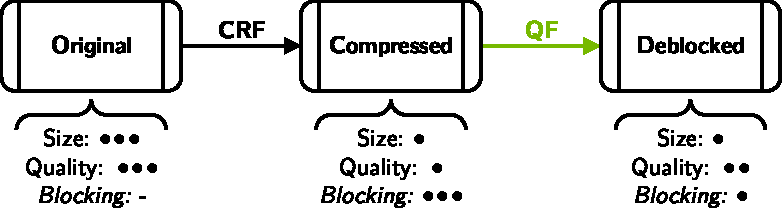
\includegraphics[width=\linewidth,keepaspectratio]{compression.pdf}
    \end{center}
    
    \[\text{CRF}=0\dots 23\dots 51\longleftrightarrow\textcolor{NvidiaGreen}{\text{QF}=1\dots 127\dots 255}\]
\end{frame}

\begin{frame}{\textcolor{NvidiaGreen}{Iteration timeline}}
    \begin{columns}[c]
        \column{0.5\linewidth}
            \centering
            \begin{enumerate}
                \item Input \texttt{>>} Frame
                \item BGR $\rightarrow$ YCrCb
                \item JPEG$\hspace{0.1 em}\triplerightarrow\hspace{0.1 em}$Luma/Chroma
                \item \textit{HostToDevice}
                \item Horizontal pass
                \item \textbf{Intermediate frame}
                \item Vertical pass
                \item \textit{DeviceToHost}
                \item Luma/Chroma $\Rrightarrow$ JPEG
                \item YCrCb $\rightarrow$ BGR
                \item Frame \texttt{>>} Output
            \end{enumerate}
        \column{0.5\linewidth}
            \centering
            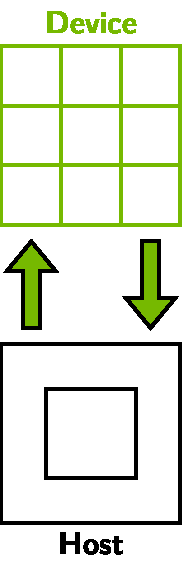
\includegraphics[height=\dimexpr\textheight-4\baselineskip-\abovecaptionskip-\belowcaptionskip\relax,keepaspectratio]{architecture.pdf}
    \end{columns}
\end{frame}

\begin{frame}{\textcolor{NvidiaGreen}{Proposed algorithm}}
    \begin{columns}[c]
        \column{0.5\linewidth}
            \centering
            \begin{algorithm}[H]
                \eIf{$|B-C|<5\wedge|D-E|<5$}
                {
                    \If{$|C-D|<(2.0\cdot \mathsf{QF})$}
                    {
                         $x\gets D-C$\;
                         $a\gets A+\frac{x}{8}$;
                         $b\gets B+\frac{x}{4}$\;
                         $c\gets C+\frac{x}{2}$;
                         $d\gets D-\frac{x}{2}$\;
                         $e\gets E-\frac{x}{4}$;
                         $f\gets F-\frac{x}{8}$\;
                    }
                }{
                    \If{$|C-D|<(0.8\cdot \mathsf{QF})$}
                    {
                         $x\gets D-C$\;
                         $b\gets B+\frac{x}{8}$;
                         $c\gets C+\frac{x}{2}$\;
                         $d\gets D-\frac{x}{2}$;
                         $e\gets E-\frac{x}{8}$\;
                    }
                }
            \end{algorithm}
        \column{0.5\linewidth}
            \centering
             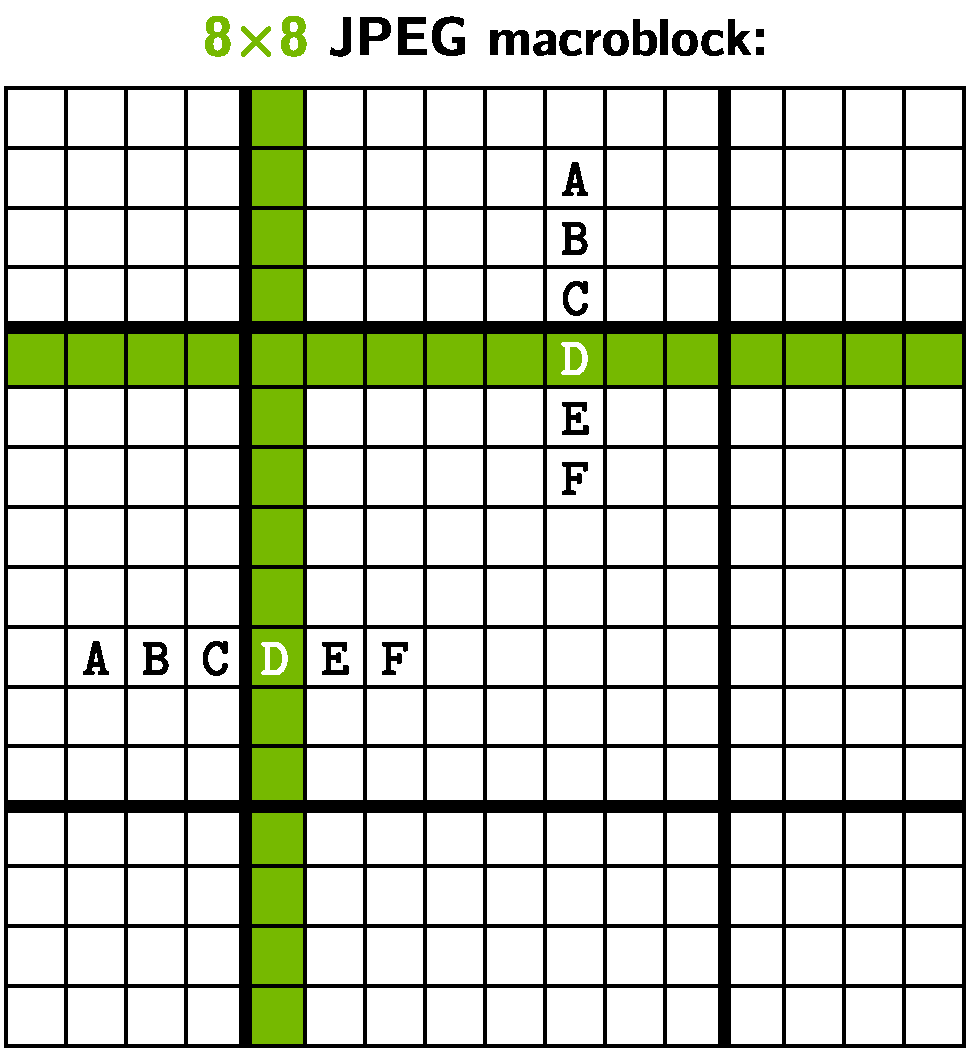
\includegraphics[height=\dimexpr\textheight-4\baselineskip-\abovecaptionskip-\belowcaptionskip\relax,keepaspectratio]{macroblock2.pdf}
    \end{columns}
\end{frame}

\begin{frame}{\textcolor{NvidiaGreen}{8-bit saturation}}
    \begin{center}
        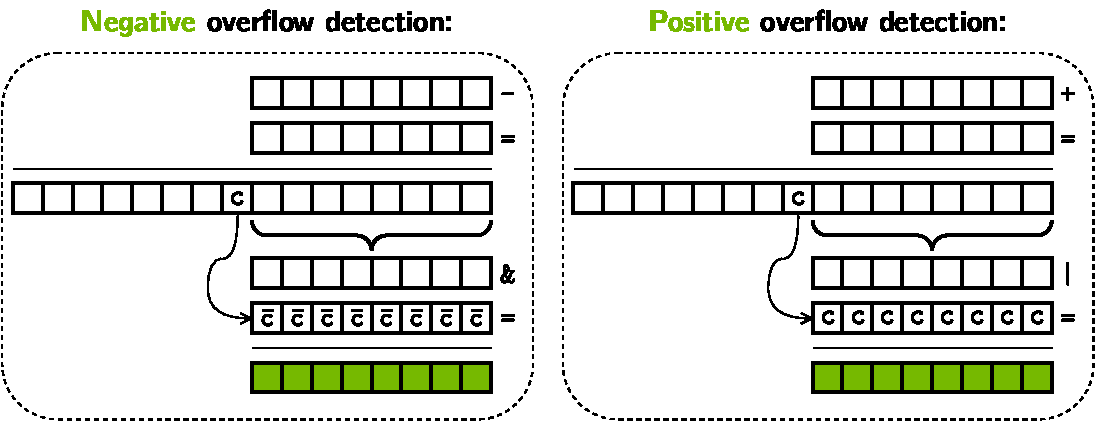
\includegraphics[width=\linewidth,keepaspectratio]{saturation.pdf}
    \end{center}

    \[A,\,B,\,C,\,D,\,E,\,F=0\dots 255\]
\end{frame}

\begin{frame}{\textcolor{NvidiaGreen}{Execution flow}}
    \begin{columns}[T]
    \column{0.49\linewidth}
        \centering
        \textbf{Synchronous host:}
        \begin{enumerate}
            \item Sample current tick
            \item Evaluate $1$ pixel \underline{alone}
            \item Repeat for $W\cdot H$ times
            \item Repeat for $3$ channels
            \item Accumulate elapsed time
            \item Restart for second pass
            \item[$\circlearrowleft$] \textit{Until no frames left}
        \end{enumerate}
    \column{0.01\linewidth}
        \centering
        \rule{0.2mm}{0.7075\textheight}
    \column{0.49\linewidth}
        \centering
        \textbf{Asynchronous \textcolor{NvidiaGreen}{device}:}
        \begin{enumerate}
            \item Upload $3$ channels
            \item Wait for $3$ events
            \item Accumulate elapsed time
            \item Evaluate $W\cdot H$ pixels \underline{simultaneously}
            \item Wait for $3$ events
            \item Accumulate elapsed time
            \item Repeat evaluation for second pass
            \item Download $3$ channels
            \item Wait for $3$ events
            \item Accumulate elapsed time
            \item[$\circlearrowleft$] \textit{Until no frames left}
        \end{enumerate}
    \end{columns}
\end{frame}

\begin{frame}{\textcolor{NvidiaGreen}{Performance improvements}}
    At least \textcolor{NvidiaGreen}{\Huge{$\bm{300\%\text{\texttt{+}}}$}} faster than the CPU, depending on:
    \begin{itemize}
        \item[\textcolor{NvidiaGreen}{\textbullet}] GPU architecture
        \item[\textcolor{NvidiaGreen}{\textbullet}] number of SMs
        \item[\textcolor{NvidiaGreen}{\textbullet}] video format
        \item[\textcolor{NvidiaGreen}{\textbullet}] stream length
        \item[\textcolor{NvidiaGreen}{\textbullet}] framerate
        \item[\textcolor{NvidiaGreen}{\textbullet}] resolution
        \item[\textcolor{NvidiaGreen}{\textbullet}] original CRF
        \item[\textcolor{NvidiaGreen}{\textbullet}] selected QF
    \end{itemize}
    to obtain \underline{the same} end result$\implies$\textit{always} the superior choice.
\end{frame}

\end{document}
